\definecolor{olifantblue}{HTML}{2A78D6}
\definecolor{olifantgreen}{HTML}{008300}
\definecolor{olifantviolet}{HTML}{4A3AA7}
\definecolor{olifantred}{HTML}{E34948}
\definecolor{olifantgray}{HTML}{666666}

\begin{figure}[t]
\centering
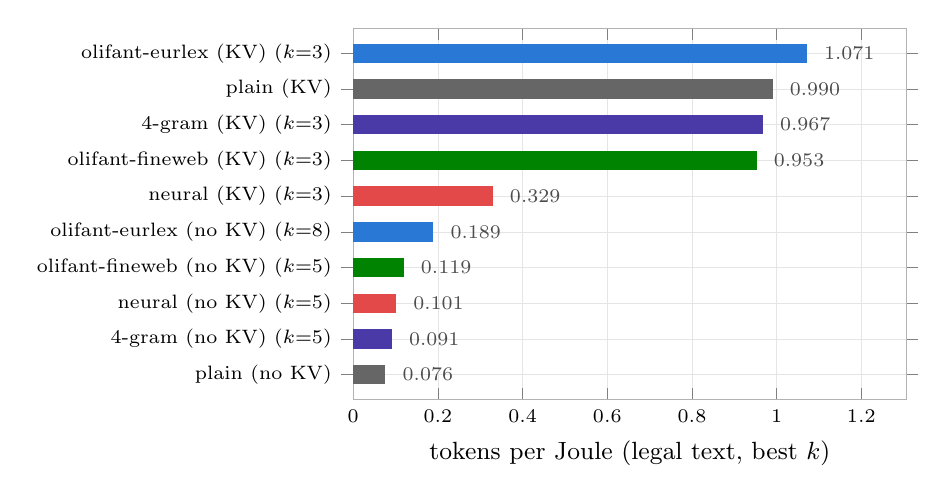
\begin{tikzpicture}
\begin{axis}[
    width=0.71\columnwidth, height=6.3cm,
    xbar, xmin=0, enlarge x limits={upper, value=0.22},
    ymin=-0.7, ymax=9.7,
    clip=false,
    xticklabel style={/pgf/number format/fixed, /pgf/number format/precision=2},
    ytick={0,1,2,3,4,5,6,7,8,9},
    yticklabels={{plain (no KV)},{4-gram (no KV) ($k$=5)},{neural (no KV) ($k$=5)},{olifant-fineweb (no KV) ($k$=5)},{olifant-eurlex (no KV) ($k$=8)},{neural (KV) ($k$=3)},{olifant-fineweb (KV) ($k$=3)},{4-gram (KV) ($k$=3)},{plain (KV)},{olifant-eurlex (KV) ($k$=3)}},
    tick label style={font=\scriptsize},
    xlabel={tokens per Joule (legal text, best $k$)},
    label style={font=\small},
    axis line style={gray!60},
    grid=major, grid style={gray!20, very thin},
    y dir=normal,
]
\addplot+[xbar, bar shift=0pt, bar width=7pt, draw=none, fill=olifantgray] coordinates { (0.0761,0) };
\addplot+[xbar, bar shift=0pt, bar width=7pt, draw=none, fill=olifantviolet] coordinates { (0.0910,1) };
\addplot+[xbar, bar shift=0pt, bar width=7pt, draw=none, fill=olifantred] coordinates { (0.1011,2) };
\addplot+[xbar, bar shift=0pt, bar width=7pt, draw=none, fill=olifantgreen] coordinates { (0.1192,3) };
\addplot+[xbar, bar shift=0pt, bar width=7pt, draw=none, fill=olifantblue] coordinates { (0.1892,4) };
\addplot+[xbar, bar shift=0pt, bar width=7pt, draw=none, fill=olifantred] coordinates { (0.3295,5) };
\addplot+[xbar, bar shift=0pt, bar width=7pt, draw=none, fill=olifantgreen] coordinates { (0.9528,6) };
\addplot+[xbar, bar shift=0pt, bar width=7pt, draw=none, fill=olifantviolet] coordinates { (0.9674,7) };
\addplot+[xbar, bar shift=0pt, bar width=7pt, draw=none, fill=olifantgray] coordinates { (0.9903,8) };
\addplot+[xbar, bar shift=0pt, bar width=7pt, draw=none, fill=olifantblue] coordinates { (1.0713,9) };
\node[right, font=\scriptsize, text=black!70] at (axis cs:0.0761,0) {~0.076};
\node[right, font=\scriptsize, text=black!70] at (axis cs:0.0910,1) {~0.091};
\node[right, font=\scriptsize, text=black!70] at (axis cs:0.1011,2) {~0.101};
\node[right, font=\scriptsize, text=black!70] at (axis cs:0.1192,3) {~0.119};
\node[right, font=\scriptsize, text=black!70] at (axis cs:0.1892,4) {~0.189};
\node[right, font=\scriptsize, text=black!70] at (axis cs:0.3295,5) {~0.329};
\node[right, font=\scriptsize, text=black!70] at (axis cs:0.9528,6) {~0.953};
\node[right, font=\scriptsize, text=black!70] at (axis cs:0.9674,7) {~0.967};
\node[right, font=\scriptsize, text=black!70] at (axis cs:0.9903,8) {~0.990};
\node[right, font=\scriptsize, text=black!70] at (axis cs:1.0713,9) {~1.071};
\end{axis}
\end{tikzpicture}
\caption{Energy efficiency ladder on legal text (tokens generated per Joule,
best $k$ per strategy). KV caching is the largest single lever; domain-matched
memory-based drafting adds to it, while the neural draft costs energy in the
cached regime.}
\label{fig:ladder}
\end{figure}
